\documentclass[11pt]{amsart}
\usepackage{amsmath}
\usepackage{geometry}                % See geometry.pdf to learn the layout options. There are lots.
\geometry{letterpaper}                   % ... or a4paper or a5paper or ... 
%\geometry{landscape}                % Activate for for rotated page geometry
%\usepackage[parfill]{parskip}    % Activate to begin paragraphs with an empty line rather than an indent
\usepackage{graphicx}
\usepackage{caption}
\usepackage{subcaption}
\usepackage{amssymb}
\usepackage{epstopdf}
\usepackage[]{algorithm2e}

\graphicspath{{../Figures/}}

\DeclareGraphicsRule{.tif}{png}{.png}{`convert #1 `dirname #1`/`basename #1 .tif`.png}

\newcommand{\vek}[1]{\mathbf{#1}}
\newcommand{\norm}[1]{\left\lVert#1\right\rVert}

\title{COMP 652: Assignment 1}
\author{Carlos G. Oliver \\ 260425853}
\date{\today}                                           % Activate to display a given date or no date

\begin{document}
\maketitle
\section{Regression}
\subsection{Q1 (c):Objective for logistic regression with $L_{2}$ regulariztion.}

The logistic regression objective is the cross entropy error function between true outputs $y_i$ and predictions $h(x_i)$ with the additional regularization term proportional to some constant $\lambda$ and the $L_2$ norm of the weight vector $\vek{w}$.
\begin{equation}
J_{\vek{w}} =  -\bigg(\sum_{i=1}^{m} y_{i}\log(h(\vek{x_{i}})) + (1 - y_{i})\log(1 - h(\vek{x_{i}}))\bigg) + \frac{\lambda}{2}\vek{w}^T\vek{w}
\end{equation}

\subsection{Q1 (d): Regularization}

For all subsequent experiments, I present summary statistics of K-fold cross validation with shuffled input data. We compute a value of $K$ so as to have approximately a training-test split ratio of $80-20\%$. This resulted in $4$ splits. The bars one each point represent one standard deviation from the mean over the $4$ splits. It is important to note that for the dataset in this assignment, the parameter space (314) is much larger than the number of instances (94) so we expect our models to display high variability. And indeed this is what we see when plotting the variance seen in K-fold cross validation {\bf Fig. ~\ref{fig:1d}}. Despite the strong variability, we are still able to note key trends in the effect of regularization strength where higher $\lambda$ appears to minimize cross entropy. The effect of lambda on the weight vector can also be noted in {\bf Fig. ~\ref{fig:1dnorm}, ~\ref{fig:1dvals}} where stronger regularization reduces the norm of the weight vector (although never to zero as we are in L2 regularization) and the values of each parameters can also be seen to converge to zero as we increase regularization strength. Overall, given the high variability in the data, it will be interesting to attempt experiments with even higher regularization strength.

\begin{figure}[h!]
    \centering
    \begin{subfigure}{0.45\textwidth}
        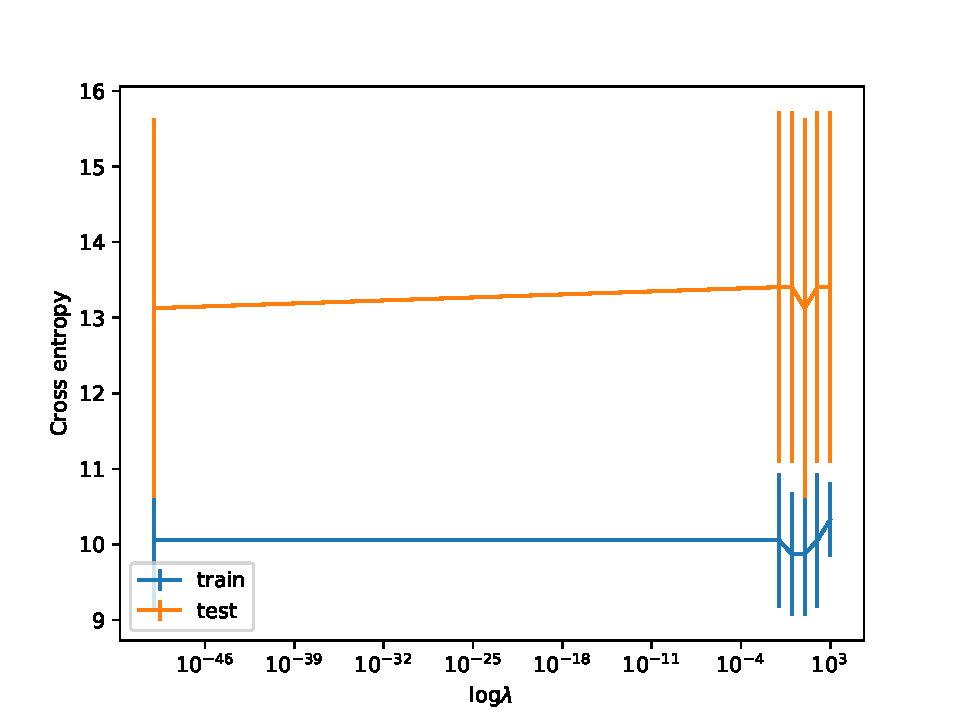
\includegraphics[width=\textwidth]{q1d_crossentropy.pdf}
        \caption{Cross entropy error over regularization strength}
        \label{fig:rnamutsnomfe_freq}
    \end{subfigure}
    \begin{subfigure}{0.45\textwidth}
        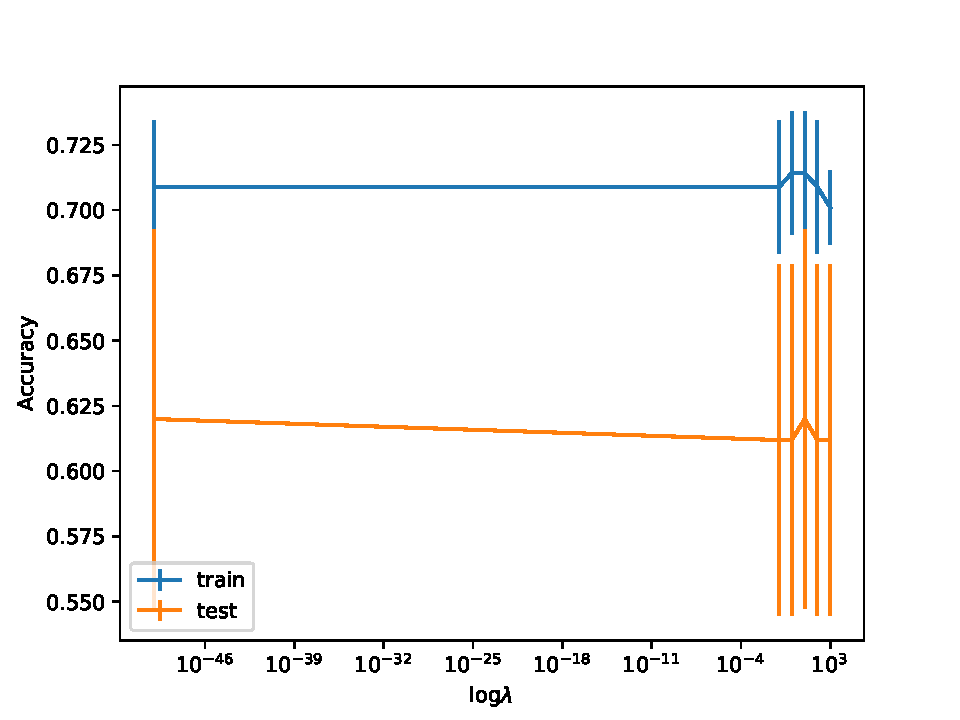
\includegraphics[width=\textwidth]{q1d_accuracy.pdf}
        \caption{Accuracy over regularization strength}
        \label{fig:ranmutsnomfe_freq}
    \end{subfigure}
    \begin{subfigure}{0.45\textwidth}
        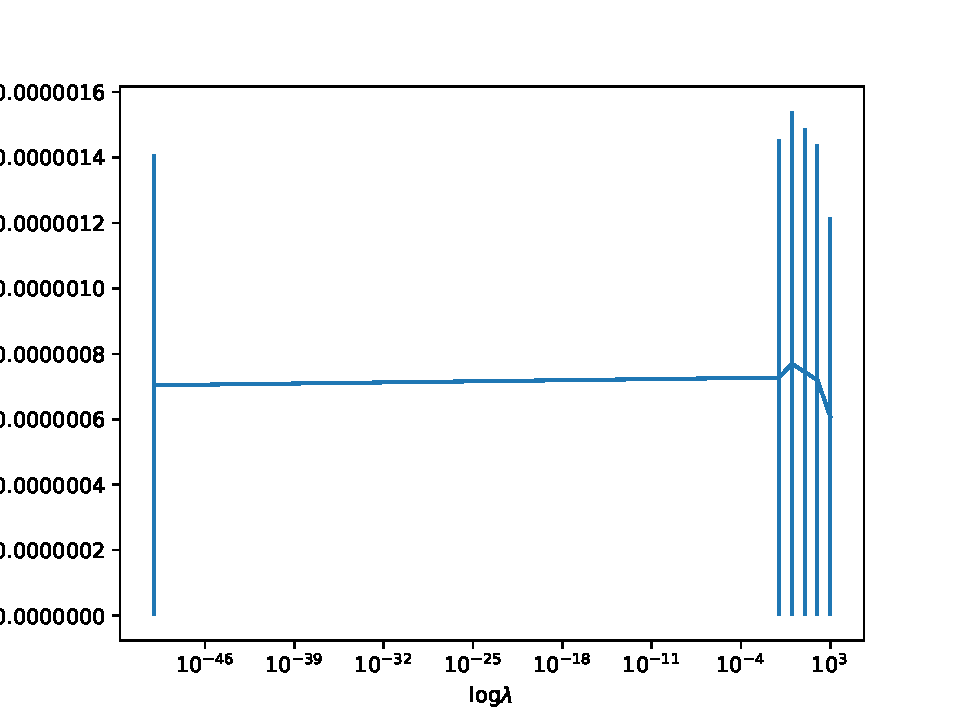
\includegraphics[width=\textwidth]{q1d_norm.pdf}
        \caption{Norm of weight vector over regularization strength}
        \label{fig:1dnorm}
    \end{subfigure}
    \begin{subfigure}{0.45\textwidth}
        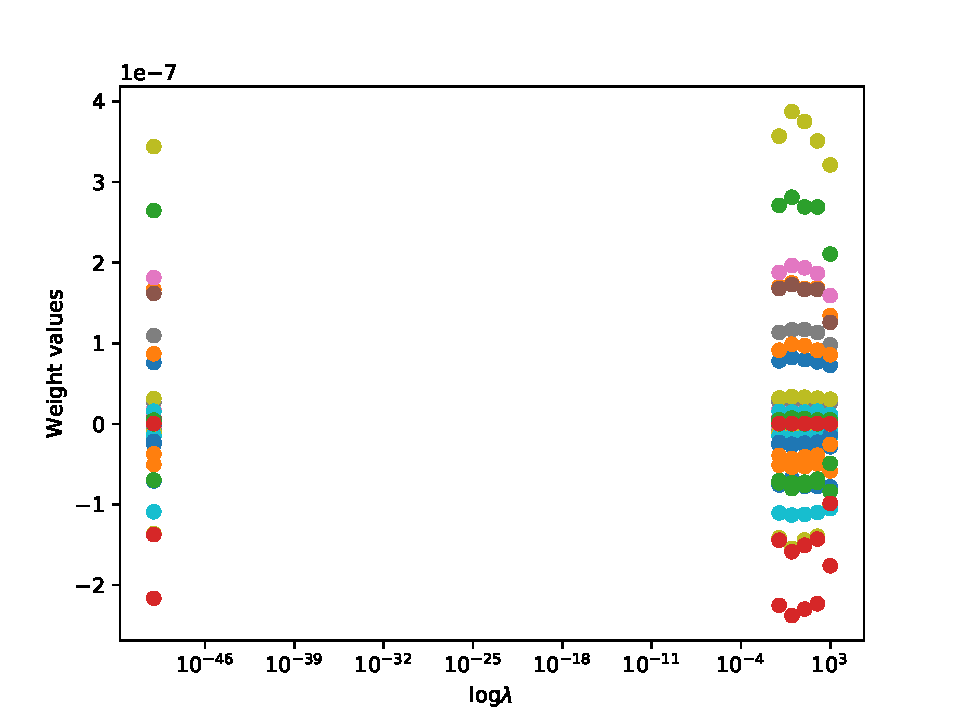
\includegraphics[width=\textwidth]{q1d_weights.pdf}
        \caption{Weight vector values over regularization strength}
        \label{fig:1dvals}
    \end{subfigure}
        \caption{Effect of regularization strength on logistic regression fitting}
    \label{fig:1d}
\end{figure}


\subsection{Q1 (e): Gaussian Basis Functions}

Next, we apply a univariate Gaussian basis function $\phi_j(x_i)$ to each value in input vectors $x$ to compute a new feature mapping. Where

\begin{equation}
	\phi(x)_j = exp\bigg[{\frac{(x_i - \mu_k)^2}{2\sigma^2}}\bigg]
\end{equation}

We apply this basis with a fixed $\sigma$ chosen from the set $\{0.1, 0.5, 1, 5, 10\}$ at each iteration. For each variable we compute $5$ basis functions ($\phi_{1}(x), ... \phi_{5}(x)$) with $\mu \in \{-10, -5, 0, 5, 10\}$ resulting in 5 feature vectors for each original feature vector in $X$. This results in a new input matrix $\Phi$.

\subsection{Q1 (f): Effect of $\sigma$ on regression}

In principle, a larger $\sigma$ should have an effect on the variance and bias of the model. A smaller sigma will result in strong penalties for points that are somewhat far from the center and thus increase the variance of the model to new data points. Interestingly, we note a strong increase in accuracy over all values of $\sigma$ see {\bf Fig. ~\ref{fig:q1f}}. This is likely due to the fact that the basis function is allowing us to better capture the complexity in the data, and indeed we see that the training accuracy reaches 100\%.

\begin{figure}[h!]
	\centering
	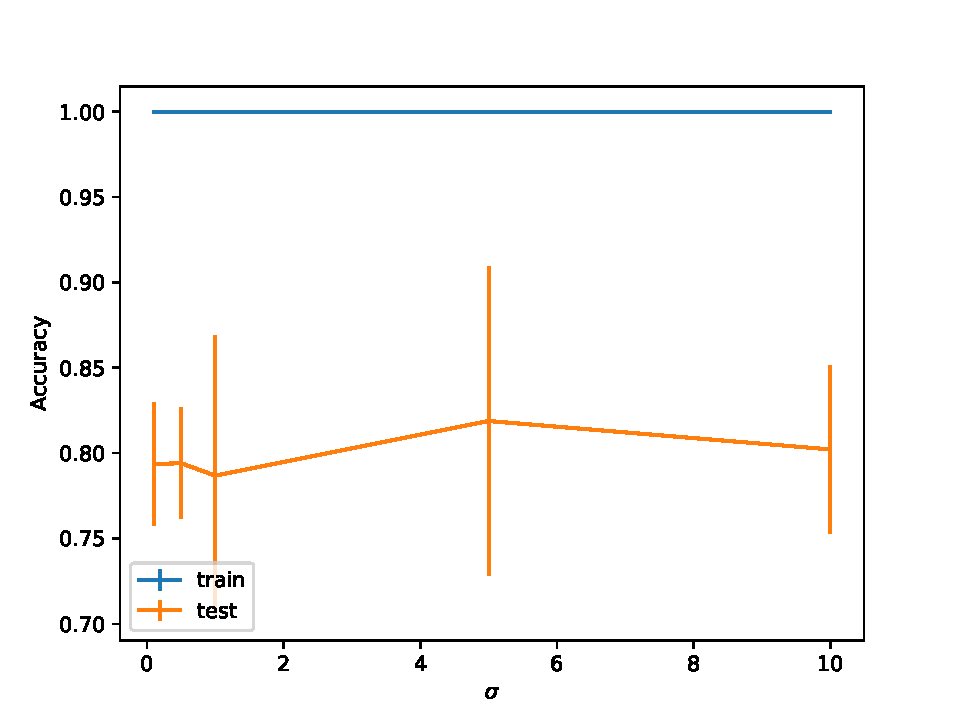
\includegraphics[width=0.45\textwidth]{sigmas.pdf}
	\caption{Fixed mean basis regression}
	\label{fig:q1f}
\end{figure}

\subsection{Q1 (g): Basis function and regularization}

Now we add in all the basis functions for each values of $\mu$ and $\sigma$ and perform logistic regression on this expanded feature space {\bf Fig. ~\ref{fig:q1g}}. We note that although cross entropy appears to also have decreased from the original input space, we notice that stronger regularization is instead producing higher cross entropy. Again, we are able to observe the decrease in the L2 norm of weight vectors across all $\sigma$ basis functions {\bf Fig. ~\ref{fig:q1f_sigmanorms}}.

\begin{figure}[h]
	\centering
		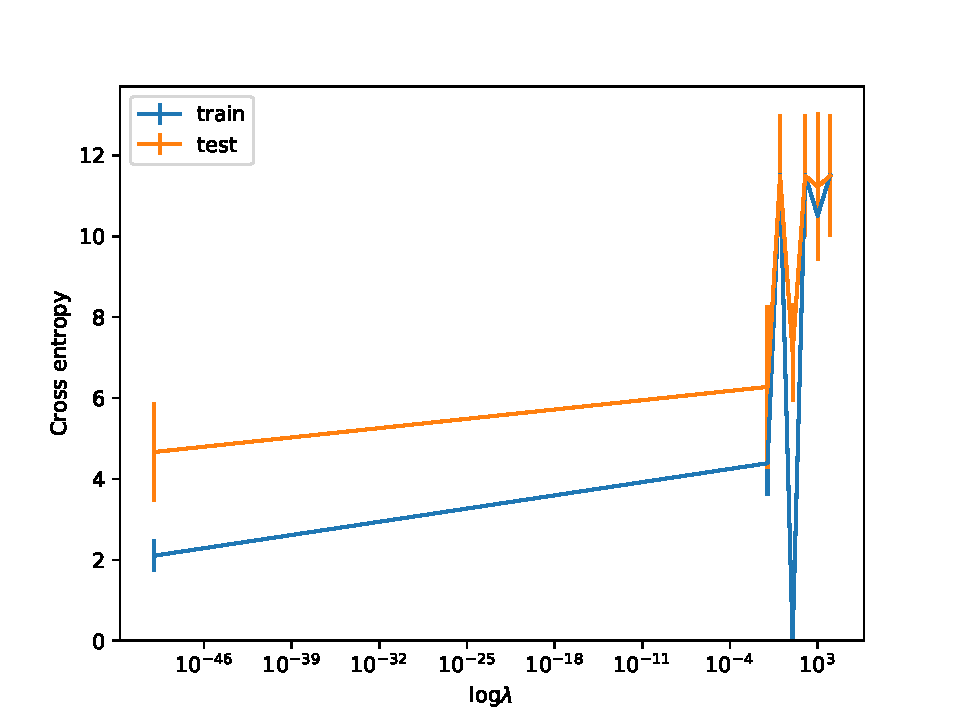
\includegraphics[width=0.45\textwidth]{all_sigmas.pdf}
		\caption{Average cross entropy with all basis functions}
		\label{fig:q1g}
\end{figure}

\begin{figure}
		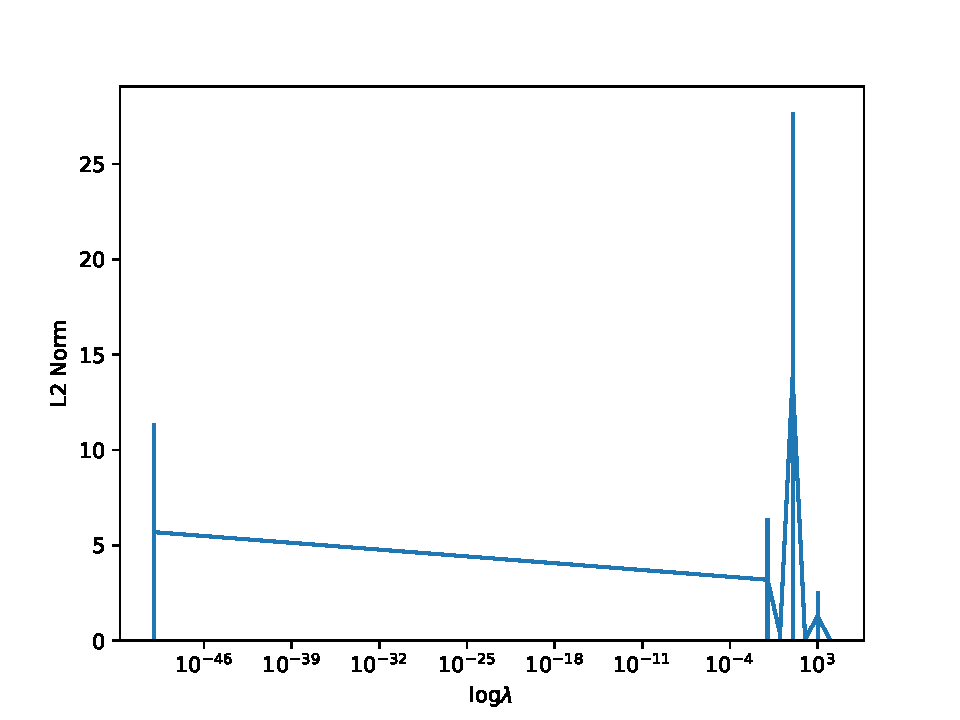
\includegraphics[width=0.45\textwidth]{all_sigmas_norm.pdf}
		\caption{L2 norm of weight vector}
\end{figure}

\begin{figure}[h!]
	\centering
	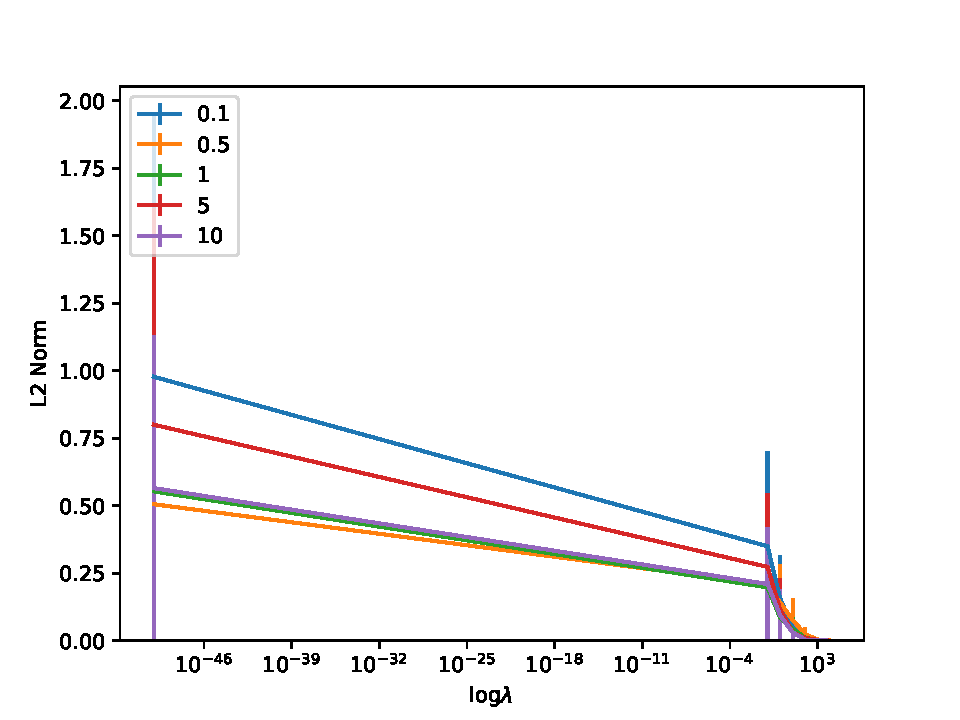
\includegraphics[width=0.45\textwidth]{all_sigma_norms.pdf}
	\caption{Full feature mapping $\sigma$ L2 norms}
	\label{fig:q1f_sigmanorms}
\end{figure}

\subsection{Q1 (h): Gaussian basis function capturing relationship between inputs}

Instead of using a univariate Gaussian basis function to transform each input variable, we could use multivariate Gaussians to capture the relationship between inputs as covariance. We can use a similar basis as before, but introduce a covariance parameter matrix $\Sigma$ that can be estimated from the data. As we would be increasing the complexity of our model, we are likely to reduce the bias but make the model more sensitive to variations in the data. 

\subsection{Q1 (i): Adaptive gaussian center placement}

Previously, we have been externally fixing the centers $\mu_i$ of the Gaussian basis functions. We can instead use the data to adaptively compute the placement of these centers. This would effectively be a clustering task, where each cluster would define the center of a Gaussian basis. With a fixed $\sigma$, the only parameter we need to estimate is the center vector $\mu$ for each center $k$. Our basis functions would then take the form:

\begin{equation}
\phi(\vek{x}) = exp\bigg(\frac{\norm{\vek{x} - \mathbf{\mu}}_2^2}{2\sigma_k^2}\bigg)
\end{equation}

We can iterate over all possible values of $k$ and keep the best performing model. 

\IncMargin{1em}
\begin{algorithm}[H]
	\SetKwInOut{Input}{input}\SetKwInOut{Output}{output}
	\SetKwFunction{KMeans}{KMeans}
	\SetKwFunction{GaussianBasis}{GaussianBasis}
	\SetKwFunction{LogisticRegression}{LogisticRegression}
	\SetKwFunction{accuracy}{accuracy}

	\Input{X, $\lambda$, $\vek{y}$, [$\sigma_0$, ..., $\sigma_j$]}
	\Output{$\vek{\omega}$}
	
	$minTestErr = \infty$\;
	$bestModel \leftarrow Null$\;
	\For{$k$ in $K$}{
		$\mu_1, ..., \mu_j \leftarrow$ \KMeans{X, k}\; 
		$X^{'} \leftarrow$ \GaussianBasis{$X, [\mu_1, ..., \mu_k]$}\;
		$model, \vek{w} \leftarrow$ \LogisticRegression{$X^{'}, y, \lambda$}\;
		$currentTestErr \leftarrow \accuracy{model, X, y}$\;
		\uIf{$currentTestErr < minTestErr$}{
			$bestModel \leftarrow model$
		}

	}
	\Return $bestModel$

\end{algorithm}

\subsection{Q1 (j): Convergence of algorithm}

We can expect this algorithm to converge to a global minimum with a proper optimization scheme, as the parametrization of logistic regression remains untouched and we can still used gradient based methods to solve the convex problem. The K-means procedure is simply a method for obtaining a feature mapping that is adaptive to the data and is an instance of expectation maximization algorithms.

\subsection{Q2 (a): Dual view of logistic regression}

The hypothesis $h(\vek{x})$ in logistic regression takes the form:

\begin{equation}
h(\vek{x}) = P(Y=1 \vert \vek{x}, \vek{w}) = \frac{1}{1 + e^{\vek{w^T}\vek{x}}}
\end{equation}

If we wish to obtain the probability distribution of $y$ condition on $\vek{x}$ and $\vek{w}$ we get:

\begin{equation}
p(y \vert \vek{x}, \vek{w}) = \sigma(y\vek{w^T}\vek{x}) = \frac{1}{1 + e^{-y\vek{w^T}\vek{x}}}
\end{equation}

We can then use this form to find the parameters that maximize the log likelihood of the data given a choice of model. (The following derivation is based on work published by Thomas P. Minka in 2007 \cite{minka2003comparison}.)

\begin{equation}
l(\vek{w}) = \sum_{i=1}^{m} \log\sigma(-y_i\vek{w^T}\vek{x}) - \frac{\lambda}{2}\vek{w^T}\vek{w}
\end{equation}

In order to derive a dual expression of this objective, we aim to find a tight linear upper bound parametrized by a new set of parameters $\alpha_{i}$. Such a function will let us reverse the order of the optimization while maintaining the same optima. In our case, if we wish to maximize $l(\vek{w})$ we can instead minimize some function $l(\vek{w}, \vek{\alpha})$ that is an upper bound to the first. We can then find the minimal value of $l(\vek{w}, \vek{\alpha})$ that maximizes $l(\vek{w})$.

We use the function:

\begin{equation}
H(\alpha) = -\alpha\log\alpha - (1-\alpha)\log(1-\alpha), \quad \alpha \in [0, 1]
\end{equation}

Plotting $H(x)$ we see that the function is quadratic.

\begin{figure}[h]
	\centering
	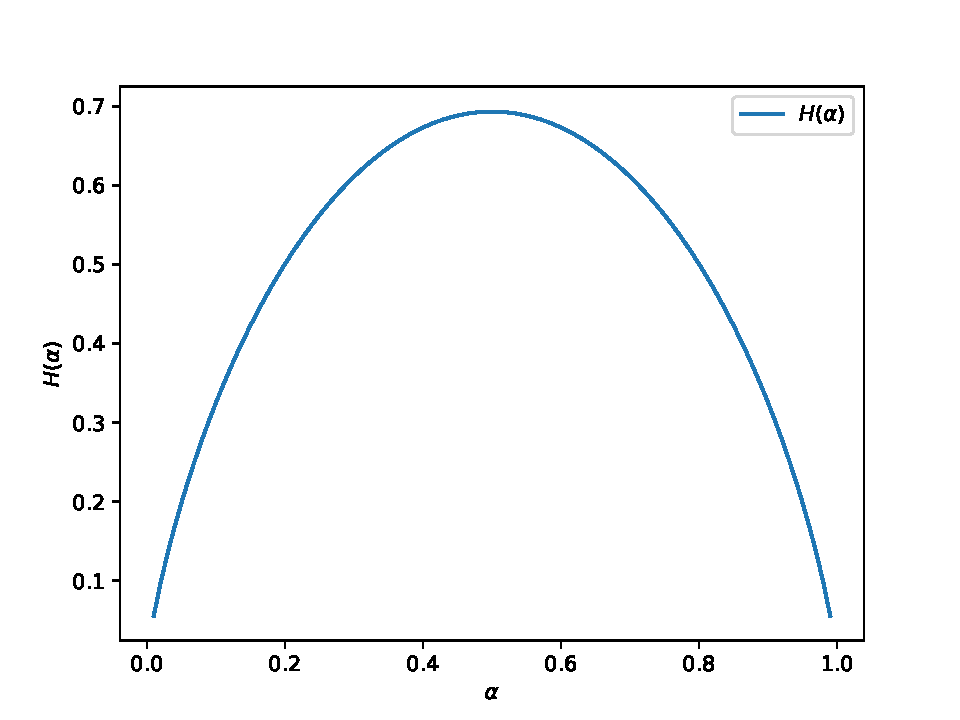
\includegraphics[width=0.45\textwidth]{H_x.pdf}
	\caption{Parameter function}
\end{figure}

Using $H(x)$ we can bound $\log(\sigma(x))$ above as follows:

\begin{equation}
\log\sigma(x) \leq \alpha x - H(x)
\end{equation} 

Plotting these functions with $\alpha = \{0, 0.5, 1\}$ we see that indeed, $\log\sigma(x)$ is tightly bounded above.

\begin{figure}
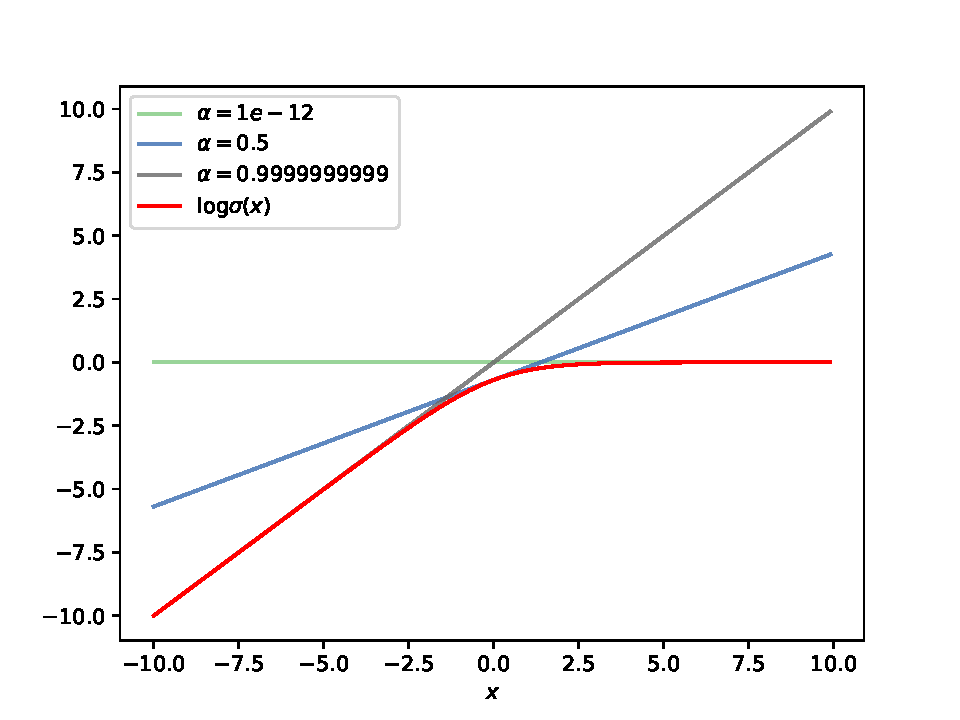
\includegraphics[width=0.45\textwidth]{bounds.pdf}
\caption{Upper bounds on log likelihood function}
\end{figure}

We can then apply these constraints to the original log likelihood function optimization problem:

\begin{equation}
l(\vek{w}) = \sum_{i}^{m} \log \sigma(y_i\vek{w^T}\vek{x}) - \frac{\lambda}{2}\vek{w^T}\vek{w} \leq l(\vek{w}, \vek{\alpha})
\end{equation}

\begin{equation}
\text{Where}\quad l(\vek{w}, \vek{\alpha}) = \sum_{i}^{m} \alpha_{i}y_{i}\vek{w^Tx_i} - H(\alpha_i) - \frac{\lambda}{2}\vek{w^Tw}
\end{equation}

We can now write the problem as a minimization problem over $\vek{\alpha}$

\begin{equation}
\min_{\alpha}\max_{\vek{w}} l(\vek{w}, \vek{\alpha})
\end{equation}

Taking the derivative of $l(\vek{w}, \alpha)$ with respect to $\vek{w}$ and setting to zero we get an expression for $\vek{w}$

\begin{equation}
\vek{w(\alpha)} = -\lambda\sum_{i}^{m}\alpha_{i}y_{i}\vek{x_i}
\end{equation}

Which we can plug into the original $l(\vek{w}, \vek{\alpha})$ and now optimize with respect to $\alpha$ to obtain

\begin{equation}
J(\vek{\alpha}) = \frac{1}{2\lambda}\sum_{i,j}^{m,n}\alpha_{i}\alpha_{j}y_{i}y_{j}\vek{x_{j}^{T}\cdot x_{i}} - \sum_{i}^{m}H(\alpha_i)
\end{equation}

This is the dual view of logistic regression, where the objective is expressed in terms of weighted dot products between input instances and not in terms of weight vector $\vek{w}$. In this form, we can apply any valid kernel to the dot product $\vek{x_i^T\cdot x_j}$ as $K(\vek{x_i, x_j)}$. It is important to note that $\vek{\alpha} \in \mathbb{R}^m$ where $m$ is the number of input instances, and $\vek{w} \in \mathbb{R}^n$ where $n$ is the number of features. When using kernel methods $n$ can grow exponentially, making the dual form more computationally tractable when the number of instances is low compared to the number of features. 

In order to solve for the optimal $\vek{\alpha}$ Minka proposes to use coordinate wise Newton method instead of Newton's method to avoid inverting the Hessian. 

\begin{equation}
g_i = \frac{dJ(\vek{\alpha})}{d\alpha_i} = y_i\vek{w(\alpha)}^T \vek{x_i} + \log \bigg(\frac{\alpha_i}{1-\alpha_i}\bigg)
\end{equation}

Using the first derivative we can iteratively step in the direction of the gradient over each $\alpha_i$.

\begin{equation}
\alpha_i^{new} = \alpha_i - \frac{g_i}{\lambda^{-1}\vek{x_i}^T\vek{x_i} + \frac{1}{\alpha_i(1-\alpha_i)}}
\end{equation}

Having obtained the vector $\vek{\alpha}$ through this procedure, we can make predictions using the original logistic model with a kernel.

\begin{equation}
P(Y=1 \vert x, \alpha) = \sigma\bigg(\sum_i^{m} \alpha_i K(\vek{x}, \vek{x_i})\bigg)
\end{equation}


\subsection{Q2 (b): Implementation of kernelized logistic regression}

Please see the \texttt{Python} script \texttt{q2.py} for a full implementation of this method.

\subsection{Q2 (c): Kernelized logistic regression vs. non-kernel logistic regression results}

I am not including results for the performance of my implementation of kernelized logistic regression as it is clear that something is not working correctly (the full code is regardless, still included in the \texttt{Src} directory). All accuracies irrespective of test or training set are around $0.3$ throughout k-fold cross validation (data not shown, see \texttt{Data} folder for data files). With more time I will continue working to fix any errors there may be in the code. However, it is also possible that the method for solving for the $\vek{\alpha}$ using the coordinate ascent I implemented is not converging adequately. I tried updating $\vek{\alpha}$ a total of 10 and 25 times with no significant increase in performance. So it is possible that many more updates are required, however this was beginning to take up a significant amount of computation time. The author in ~\cite{minka2003comparison} proposes a prioritized update scheme that might help the algorithm converge faster. 

Assuming the implementation had worked as expected, I can speculate on the performance as a function of the width of the kernel. Certainly a higher degree polynomial kernel will be more prone to overfitting which would become apparent in the increased performance on the training set as compared with the test set. The degree at which this would occur would have to be determined by cross validation. Such methods are especially well suited or the kind of dataset presented in this assignment where the feature space is much larger than the number of observations.

\begin{table}[h!]
\centering
\begin{tabular}{lll}
\hline
k-fold & Train & Test  \\ \hline
1      & 0.680 & 0.5   \\ \hline
2      & 0.691 & 0.625 \\ \hline
3      & 0.747 & 0.645 \\ \hline
4      & 0.715 & 0.677 \\ \hline
\end{tabular}
\caption{Regular Logistic Regression Accuracy $\lambda=1$}
\label{fig:q2c_reg}
\end{table}

\subsection{Q2 (d): Advantages and disadvantages of kernelized logistic regression (KLR)}
Again, since I was unable to produce interpretable data for KLR, these  responses are theoretical.

{\bf Advantages:}

\begin{itemize}
	\item The addition of kernels allows for a priori field knowledge to be coded into the models and produce more accurate models.
	\item Non-linear patterns can be modelled at relatively low computational costs
\end{itemize}

{\bf Disadvantages:}
	\begin{itemize}
	\item The computational cost associated with kernel methods scales with input size, in this example input size was quite low so computation was not very expensive. However, already with 25 updates on $\alpha$ the slowdown was noticeable. Many data sets might include much larger data instances and computation will be much more costly.
	\end{itemize}
\subsection{Q3: (a) Kernels}

{\it Statement:} $K(\vek{x}, \vek{z}) = aK_1(\vek{x}, \vek{z}) + bK_{2}(\vek{x}, \vek{z})$ is a kernel given that $K_1$ and $K_2$ are kernels and $a,b \in \mathbb{R}$ and $a, b > 0$.

\begin{proof}

If $K_1$ and $K_2$ are kernels then we can write them as:

\begin{equation}
K_1(\vek{x}, \vek{z}) = \phi^1(\vek{x})^T\phi^1(\vek{z})
\end{equation}

\begin{equation}
K_2(\vek{x}, \vek{z}) = \phi^2(\vek{x})^T\phi^2(\vek{z})
\end{equation}


We define two new feature mappings $\phi^a(\vek{x})$ and $\phi^b(\vek{x})$ which are scalar products of the original $\phi(\vek{x})$.

\begin{equation}
\phi^a(\vek{x}) = (\sqrt{a}x_1, \sqrt{a}x_2...\sqrt{a}x_n)
\end{equation}

\begin{equation}
\phi^b(\vek{x}) = (\sqrt{b}x_1, \sqrt{b}x_2...\sqrt{b}x_n)
\end{equation}

Taking their dot products we can construct a new kernel $K^a(\vek{x}, \vek{z})$

\begin{equation}
K^a(\vek{x}, \vek{z}) = \phi^a(\vek{x})^T \cdot \phi^a(\vek{z}) = (\sqrt{a}\sqrt{a}x_1 z_1 + \sqrt{a}\sqrt{a}x_2 z_2 + ... \sqrt{a}\sqrt{a}x_n z_n ) = aK^2(\vek{x}, \vek{z})
\end{equation}

We can do the same for $\phi^b({\vek{x}})$.

By conctatenating feature maps $\phi^{a}(\vek{x})$ and $\phi^{b}(\vek{x})$ into $\phi(\vek{x})$ we can express $aK_1 + bK_2$ as a dot product of this new feature map.

\begin{equation}
\phi(\vek{x})^T \cdot \phi(\vek{z}) = (\sqrt{a}\phi^a(x_1)\sqrt{a}\phi^a(x_1) + \sqrt{a}\phi^a(x_1)\sqrt{a}\phi^a(x_1) + ... + \sqrt{b}\phi^b(x_1)\sqrt{b}\phi^b(x_1) + \sqrt{b}\phi^b(x_1)\sqrt{b}\phi^b(x_1) + ... )
\end{equation}

Which reduces to 

\begin{equation}
K(\vek{x}, \vek{z}) = \phi^{a}(\vek{z})^T \cdot \phi^{b}(\vek{z})
\end{equation}

\end{proof} 

\subsection{Q3 (b) Kernels}

{\it Statement: } $K(\vek{x}, \vek{z}) = K_1(\vek{x}, \vek{z})K_2(\vek{x}, \vek{z})$

\begin{proof}

This proof is based on the proof for the product of kernels in the Bishop textbook Ch. 6. ~\cite{bishop2006pattern}.

We can expand each kernel into dot products of their respective feature vectors $\phi^{1}$ and $\phi^{2}$

\begin{equation} 
\begin{split}
K(\vek{x}, \vek{z}) & =  (\phi^1(\vek{x})^T \cdot \phi^1(\vek{z}))(\phi^2(\vek{x})^T \cdot \phi^2(\vek{z}))\\
 & = \sum_{i,j} \phi_i^1(\vek{x})\phi_j^2(\vek{x}) \phi_i^1(\vek{z})\phi_j^2(\vek{z})
\end{split}
\label{eq:kern}
\end{equation}

To show that this is a kernel, we need to write it as the dot product of two feature mappings. We define a new feature map $\phi^{'}_{i,j}(\vek{x}) = \phi^{1}_i(\vek{x}) \phi^2_j(\vek{x})$ that yields a feature for each pair $i$, $j$ in $\vek{x}$. We now plug this expression back in to (\ref{eq:kern}) to obtain:

\begin{equation}
K(\vek{x}, \vek{z}) = \phi^{'}(\vek{x})\phi^{'}(\vek{z})
\end{equation}

\end{proof}

\bibliographystyle{unsrt}
\bibliography{bibliography}


\end{document}  
